%!TEX root = ../dissertation.tex

\chapter{Генерация всех неизоморфных детерминированных конечных автоматов, удовлетворяющих заданным примерам поведения} 
\label{sec:findall}

В данной главе рассматривается задача генерации всех неизоморфных детерминированных конечных автоматов минимального размера, соответствующих заданным примерам поведения, которая ранее не имела эффективного решения.
Разрабатывается метод, основанный на подходе к решению задачи генерации одного ДКА с использованием программных средстве решения SAT, подробно описанный в разделе~\ref{sec:review:sat-dfa-inf}.
Рассматриваются два варианта использования программных средств решения SAT: перезапуск неинкрементального средства после нахождения каждого автомата и использование инкрементального средства~{---} если такое средство находит некоторое решение, то оно сохраняет свое текущее состояние и может принимать новые дизъюнкты.
Подробнее про инкрементальное решение SAT можно прочитать в~\cite{DBLP:conf/sat/EenS03}.
Также в данной главе предлагается переборный метод, который служит базовым для сравнения с методом, основанным на сведении к задаче выполнимости.

%----------------------------------------------------------------------------------------

\section{Мотивация и постановка задачи}
\label{sec:findall:problem}

В классической задаче генерации ДКА по заданным примерам поведения (см. раздел~\ref{sec:review:dfa-inf:task}) ищется некоторый детерминированный конечный автомат минимального размера, соответствующий имеющимся примерам.
Однако, вполне возможна ситуация, когда одному и тому же набору примеров поведения соответствует более одного ДКА минимального размера $M$.
Как было описано в разделе~\ref{sec:review:dfa-inf:isomorphic-automata} для каждого автомата $\mathcal{D}$ размера $M$ существует $\mathcal{O}\left(M\right)$ изоморфных ему автоматов.
Но изоморфные автоматы задают один и тот же язык, поэтому не представляют никакого интереса.
В настоящей главе рассматривается ситуация, когда существуют несколько различных, неизоморфных ДКА минимального размера, соответствующих примерам поведения.
На рисунке~\ref{img:find-all} приведены все неизоморфные ДКА минимального размера, построенные по заданным примерам поведения.

\begin{figure}[ht]
  \centering
  \ifafour
    \begin{tikzpicture}[
    ->, % makes the edges directed
    >=stealth', % makes the arrow heads bold
    node distance=1.9cm, % specifies the minimum distance between two nodes. Change if necessary.
    every state/.style={thick, fill=gray!10, minimum size = 0pt}, % sets the properties for each ’state’ node
    initial text=$ $, % sets the text that appears on the start arrow
    double distance between line centers=2pt
    ]
  \node (a1) 
    {
      \begin{tikzpicture}
        \node[state, initial]     (q11)                 {$1$};
        \node[state, accepting]   (q12) [right of=q11]  {$2$};
        \node[state]              (q13) [below of=q11]  {$3$};

        \path     (q11) edge  [above]       node {a,b}  (q12)
                  (q12) edge  [below right] node {a}    (q13)
                        edge  [loop above]  node {b}    (q12)
                  (q13) edge  [left]        node {a,b}  (q11)
                        ;
      \end{tikzpicture}
    };
  \node[right=0.1cm of a1] (a2)
    {
      \begin{tikzpicture}
        \node[state, initial, accepting]  (q21)                 {$1$};
        \node[state, accepting]           (q22) [right of=q21]  {$2$};
        \node[state]                      (q23) [below of=q21]  {$3$};

        \path     (q21) edge  [above]                 node {a,b}  (q22)
                  (q22) edge  [below right]           node {a}    (q23)
                        edge  [bend right=60, above]  node {b}    (q21)
                  (q23) edge  [left]                  node {a}    (q21)
                        edge  [loop below]            node {b}    (q23)
                        ;
      \end{tikzpicture}
    };
  \node[right=0.1cm of a2] (a3)
    {
      \begin{tikzpicture}
        \node[state, initial, accepting]  (q31)                 {$1$};
        \node[state, accepting]           (q32) [right of=q31]  {$2$};
        \node[state]                      (q33) [below of=q31]  {$3$};

        \path     (q31) edge  [above]                 node {a,b}  (q32)
                  (q32) edge  [below right]           node {a}    (q33)
                        edge  [loop above]            node {b}    (q32)
                  (q33) edge  [left]                  node {a}    (q31)
                        edge  [loop below]            node {b}    (q33)
                        ;
      \end{tikzpicture}
    };
  \node[below=0.1cm of a1] (a4)
    {
      \begin{tikzpicture}
        \node[state, initial, accepting]  (q41)                 {$1$};
        \node[state, accepting]           (q42) [right of=q41]  {$2$};
        \node[state]                      (q43) [below of=q41]  {$3$};

        \path     (q41) edge  [above]                 node {a}    (q42)
                        edge  [loop above]            node {b}    (q41)
                  (q42) edge  [below right]           node {a,b}  (q43)
                  (q43) edge  [left]                  node {a}    (q41)
                        edge  [loop below]            node {b}    (q43)
                        ;
      \end{tikzpicture}
    };
  \node[right=0.1cm of a4] (a5)
    {
      \begin{tikzpicture}
        \node[state, initial, accepting]  (q51)                 {$1$};
        \node[state, accepting]           (q52) [right of=q51]  {$2$};
        \node[state]                      (q53) [below of=q51]  {$3$};

        \path     (q51) edge  [above]                       node {a}    (q52)
                        edge  [bend right=30, left]         node {b}    (q53)
                  (q52) edge  [above left]   node {a}    (q53)
                        edge  [loop above]                  node {b}    (q52)
                  (q53) edge  [right]        node {a}    (q51)
                        edge  [bend right=30, below right]  node {b}    (q52)
                        ;
      \end{tikzpicture}
    };
  \node[right=0.1cm of a5] (a6)
    {
      \begin{tikzpicture}
        \node[state, initial]             (q61)                 {$1$};
        \node[state, accepting]           (q62) [right of=q61]  {$2$};
        \node[state]                      (q63) [below of=q61]  {$3$};

        \path     (q61) edge  [above]                       node {a}    (q62)
                        edge  [bend right=30, left]         node {b}    (q63)
                  (q62) edge  [above left]   node {a}    (q63)
                        edge  [loop above]                  node {b}    (q62)
                  (q63) edge  [right]        node {a}    (q61)
                        edge  [bend right=30, below right]  node {b}    (q62)
                        ;
      \end{tikzpicture}
    };
  \node[below=0.1cm of a4, xshift=1.8cm] (a7)
    {
      \begin{tikzpicture}
        \node[state, initial]             (q71)                 {$1$};
        \node[state, accepting]           (q72) [right of=q71]  {$2$};
        \node[state]                      (q73) [below of=q71]  {$3$};

        \path     (q71) edge  [above]                 node {a,b}  (q72)
                  (q72) edge  [below right]           node {a}    (q73)
                        edge  [loop above]            node {b}    (q72)
                  (q73) edge  [left]                  node {a}    (q71)
                        edge  [loop below]            node {b}    (q73)
                        ;
      \end{tikzpicture}
    };
  \node[right=0.1cm of a7] (a8)
    {
      \begin{tikzpicture}
        \node[state, initial, accepting]  (q81)                 {$1$};
        \node[state, accepting]           (q82) [right of=q81]  {$2$};
        \node[state]                      (q83) [below of=q81]  {$3$};

        \path     (q81) edge  [above]                       node {a}    (q82)
                        edge  [bend right=30, left]         node {b}    (q83)
                  (q82) edge  [bend left=30, below right]   node {a}    (q83)
                        edge  [loop above]                  node {b}    (q82)
                  (q83) edge  [right]        node {a,b}  (q81)
                        ;
      \end{tikzpicture}
    };
\end{tikzpicture}

  \else
    \begin{tikzpicture}[
    ->, % makes the edges directed
    >=stealth', % makes the arrow heads bold
    node distance=1.9cm, % specifies the minimum distance between two nodes. Change if necessary.
    every state/.style={thick, fill=gray!10, minimum size = 0pt}, % sets the properties for each ’state’ node
    initial text=$ $, % sets the text that appears on the start arrow
    ]
  \node (a1) 
    {
      \begin{tikzpicture}
        \node[state, initial]     (q11)                 {$1$};
        \node[state, accepting]   (q12) [right of=q11]  {$2$};
        \node[state]              (q13) [below of=q11]  {$3$};

        \path     (q11) edge  [above]       node {a,b}  (q12)
                  (q12) edge  [below right] node {a}    (q13)
                        edge  [loop above]  node {b}    (q12)
                  (q13) edge  [left]        node {a,b}  (q11)
                        ;
      \end{tikzpicture}
    };
  \node[right=0.1cm of a1] (a2)
    {
      \begin{tikzpicture}
        \node[state, initial, accepting]  (q21)                 {$1$};
        \node[state, accepting]           (q22) [right of=q21]  {$2$};
        \node[state]                      (q23) [below of=q21]  {$3$};

        \path     (q21) edge  [above]                 node {a,b}  (q22)
                  (q22) edge  [below right]           node {a}    (q23)
                        edge  [bend right=45, above]  node {b}    (q21)
                  (q23) edge  [left]                  node {a}    (q21)
                        edge  [loop below]            node {b}    (q23)
                        ;
      \end{tikzpicture}
    };
  \node[right=0.1cm of a2] (a3)
    {
      \begin{tikzpicture}
        \node[state, initial, accepting]  (q31)                 {$1$};
        \node[state, accepting]           (q32) [right of=q31]  {$2$};
        \node[state]                      (q33) [below of=q31]  {$3$};

        \path     (q31) edge  [above]                 node {a,b}  (q32)
                  (q32) edge  [below right]           node {a}    (q33)
                        edge  [loop above]            node {b}    (q32)
                  (q33) edge  [left]                  node {a}    (q31)
                        edge  [loop below]            node {b}    (q33)
                        ;
      \end{tikzpicture}
    };
  \node[below=0.1cm of a1] (a4)
    {
      \begin{tikzpicture}
        \node[state, initial, accepting]  (q41)                 {$1$};
        \node[state, accepting]           (q42) [right of=q41]  {$2$};
        \node[state]                      (q43) [below of=q41]  {$3$};

        \path     (q41) edge  [above]                 node {a}    (q42)
                        edge  [loop above]            node {b}    (q41)
                  (q42) edge  [below right]           node {a,b}  (q43)
                  (q43) edge  [left]                  node {a}    (q41)
                        edge  [loop below]            node {b}    (q43)
                        ;
      \end{tikzpicture}
    };
  \node[right=0.1cm of a4] (a5)
    {
      \begin{tikzpicture}
        \node[state, initial, accepting]  (q51)                 {$1$};
        \node[state, accepting]           (q52) [right of=q51]  {$2$};
        \node[state]                      (q53) [below of=q51]  {$3$};

        \path     (q51) edge  [above]                       node {a}    (q52)
                        edge  [bend right=10, left]         node {b}    (q53)
                  (q52) edge  [bend right=10, above left]   node {a}    (q53)
                        edge  [loop above]                  node {b}    (q52)
                  (q53) edge  [bend right=10, right]        node {a}    (q51)
                        edge  [bend right=10, below right]  node {b}    (q52)
                        ;
      \end{tikzpicture}
    };
  \node[right=0.1cm of a5] (a6)
    {
      \begin{tikzpicture}
        \node[state, initial]             (q61)                 {$1$};
        \node[state, accepting]           (q62) [right of=q61]  {$2$};
        \node[state]                      (q63) [below of=q61]  {$3$};

        \path     (q61) edge  [above]                       node {a}    (q62)
                        edge  [bend right=10, left]         node {b}    (q63)
                  (q62) edge  [bend right=10, above left]   node {a}    (q63)
                        edge  [loop above]                  node {b}    (q62)
                  (q63) edge  [bend right=10, right]        node {a}    (q61)
                        edge  [bend right=10, below right]  node {b}    (q62)
                        ;
      \end{tikzpicture}
    };
  \node[below=0.1cm of a4, xshift=1.8cm] (a7)
    {
      \begin{tikzpicture}
        \node[state, initial]             (q71)                 {$1$};
        \node[state, accepting]           (q72) [right of=q71]  {$2$};
        \node[state]                      (q73) [below of=q71]  {$3$};

        \path     (q71) edge  [above]                 node {a,b}  (q72)
                  (q72) edge  [below right]           node {a}    (q73)
                        edge  [loop above]            node {b}    (q72)
                  (q73) edge  [left]                  node {a}    (q71)
                        edge  [loop below]            node {b}    (q73)
                        ;
      \end{tikzpicture}
    };
  \node[right=0.1cm of a7] (a8)
    {
      \begin{tikzpicture}
        \node[state, initial, accepting]  (q81)                 {$1$};
        \node[state, accepting]           (q82) [right of=q81]  {$2$};
        \node[state]                      (q83) [below of=q81]  {$3$};

        \path     (q81) edge  [above]                       node {a}    (q82)
                        edge  [bend right=10, left]         node {b}    (q83)
                  (q82) edge  [below right]                 node {a}    (q83)
                        edge  [loop above]                  node {b}    (q82)
                  (q83) edge  [bend right=10, right]        node {a,b}  (q81)
                        ;
      \end{tikzpicture}
    };
\end{tikzpicture}

  \fi
  \caption{Все неизоморфные ДКА, соответствующие множествам примеров поведения $S_{+} = \left\{a, bb, aaaa\right\}$ и $S_{-}=\left\{aa, bab\right\}$}
  \label{img:find-all}
\end{figure}

Такая ситуация может возникнуть, либо если заданных примеров поведения недостаточно, чтобы точно описать целевой автомат, либо они недостаточного качества.
Например, примеров поведения очень много, но большая их часть покрывает лишь часть переходов целевого ДКА.
Тогда становится актуальной генерация всех возможных автоматов минимального размера, соответствующих заданным примерам поведения.
Имея все возможные автоматы их можно проанализировать, чтобы найти закономерности или чтобы понять, почему имеющиеся примеры поведения допускают несколько решений.
Также, нужный автомат среди всех найденных может быть выбран в дальнейшем при помощи дополнительных проверок или спецификаций.

Формально задача генерации всех ДКА формулируется аналогично задаче генерации одного автомата.
Пусть примеры поведения представлены двумя множествами слов над алфавитом $\Sigma$: $S_{+}$~--- множество слов, которые должны допускаться искомыми автоматами; $S_{-}$~--- множество слов, которые должны отвергаться искомыми автоматами.
Тогда задача генерации всех различных детерминированных конечных автоматов заключается в поиске все неизоморфных автоматов, который будут принимать все слова из $S_{+}$ и отвергать все слова из $S_{-}$.

Эвристические, метаэвристические и другие неточные методы генерации автоматов по примерам поведения не применимы для решения такой задачи, так как число находимых ими автоматов ничем не ограничено.
Точные методы генерации ДКА на основе сведения к SAT применимы для поиска всех различных автоматов, так как способны перебрать все пространство поиска и найти все автоматы минимального размера, но без применения BFS-предикатов нарушения симметрии они допускают факториал изоморфных ДКА, что не позволяет применять их на практике.
BFS-предикаты, в свою очередь, как было представлено в разделе~\ref{sec:review:sym-breaking:bfs-based}, оставляют единственного представителя для каждого класса эквивалентности по изоморфизму.
В следующем разделе предлагается первый эффективный метод для решения задачи генерации всех различных ДКА, основанный на сведении к SAT и BFS-предикатах.

Еще одним важным применением разрабатываемого метода является формальная возможность доказать единственность найденного ДКА.
Действительно, если при решении задачи генерации всех различных ДКА минимального размера генерируется единственный автомат, то можно сделать вывод, что других автоматов такого размера, соответствующих заданным примерам поведения, не существует.
Данный факт может использоваться как косвенное доказательство того, что обучающие данные подобраны достаточно хорошо и хорошо описывают найденный автомат.

%----------------------------------------------------------------------------------------

\section{Метод генерации всех неизоморфных детерминированных конечных автоматов, соответствующих заданным примерам поведения, основанный на сведении к задаче выполнимости}
\label{sec:findall:SAT-based}

Как было описано в разделе~\ref{sec:review:dfa-inf:isomorphic-automata}, для каждого ДКА с $M$ состояниями существует $\mathcal{O}\left(M!\right)$ изоморфных ему автоматов.
Основной идеей предлагаемого метода по генерации всех ДКА является запрет (блокирование) найденных удовлетворяющих подстановок.
Очевидно, что без использования предикатов нарушения симметрии, придется блокировать $\mathcal{O}\left(M\right)$ изоморфных автоматов для каждого найденного уникального ДКА, что даже при $M = 10$ требует значительных вычислительных затрат.
Так как подход к нарушению симметрии с помощью большой клики, описанный в разделе~\ref{sec:review:sat-dfa-inf:sat}, позволяет зафиксировать только нумерацию $k$ состояний, то метод, предложенный в~\cite{heule-icgi10} находит $\left(C - k\right)!$ изоморфных автоматов, что в общем случае все еще вычислительно сложно.

Предикаты нарушения симметрии на основе обхода в ширину, как было описано в разделе~\ref{sec:review:sym-breaking:bfs-based}, в свою очередь допускают единственного представителя каждого класса эквивалентности по изоморфизму.
Конкретно, BFS-предикаты допускают BFS-пронумерованный автомат.
Тогда, заблокировав единственный найденный автомат, автоматически блокируется весь класс эквивалентности, а значит далее программное средство может найти другой автомат только если он не является изоморфным ранее найденным.
Необходимо заметить, что несмотря на то, что идея блокировать найденные решения с целью найти остальные достаточно проста и известна, применять ее на практике невозможно без эффективных предикатов нарушения симметрии.
Так, ранее не было описано способов бороться с факториальным числом изоморфных автоматов, а значит и рассматриваемая задача не имела эффективного решения.
Использование BFS-предикатов позволяет решить данную задачу путем добавления \emph{блокирующего} дизъюнкта в булеву формулу. 

Как было сказано в разделе~\ref{sec:review:dfa-inf:dfa-def}, детерминированным конечным автоматом называется пятерка $\mathcal{D} = \left(D,\Sigma,\delta,d_{1},D^{+}\right)$.
При построении автомата по найденной выполняющей подстановке множество состояний $D$ задано неявно через текущее число состояний автомата $M$, алфавит $\Sigma$~{---} через число $L$, стартовое состояние $d_{1}$ всегда имеет номер $1$, функция переходов $\delta$ определяется с помощью переменных переходов $y_{i,l,j}$, а множество допускающих состояний с помощью переменных допуска $z_{i}$.
Тогда достаточно из всей найденной выполняющей подстановки запретить только значения переменных переходов и значения переменных допуска.
Если с помощью $\varphi\left(q\right)$ обозначить значение переменной $q$ в найденной подстановке $\varphi$ и определить множество $\mathcal{Y} = \{y_{i,l,j} | i,j \in \left[M\right] \wedge l \in \Sigma \wedge \varphi\left(y_{i,l,j}\right) = 1\}$, то блокирующий дизъюнкт можно определить следующим образом:
\begin{equation*}
\bigwedge_{y \in \mathcal{Y}} \neg y \wedge \bigwedge_{i \in \left[M\right]}\neg \varphi\left(z_{i}\right).
\end{equation*}


Существует два различных способа использования программных средств для решения SAT.
Во-первых, можно перезапускать неинкрементальное средство с новой булевой формулой с добавленным блокирующим дизъюнктом после каждого нахождения выполняющей подстановки.
Недостатком данного подхода является то, что процесс поиска решения каждый раз начинается заново, и программное средство каждый раз проделывает полный объем работы по перебору пространства поиска.
Второй подход основан на использовании инкрементальных программных средств, которые после нахождения выполняющей подстановки сохраняют свое состояние и способны продолжить поиск решения после добавления некоторого уточнения, выраженного одним или несколькими дизъюнктами.
Подробнее про инкрементальное решение SAT можно прочитать в~\cite{DBLP:conf/sat/EenS03}.

% \inote{возможно, добавить схему всего этого.}

Необходимо заметить, что если найдено два автомата $\mathcal{D}_1 = \left(D,\Sigma,\delta,d_{1},D_{1}^{+}\right)$ и $\mathcal{D}_2 = \left(D,\Sigma,\delta,d_{1},D_{2}^{+}\right)$, которые различаются только множествами допускающих состояний, то можно сделать вывод, что в исходных примерах поведения нет строк, определяющих допуск одного или нескольких состояний автоматов $\mathcal{D}_{1}$ и $\mathcal{D}_{2}$.
Если использовать предложенный выше блокирующий дизъюнкт, то будут найдены все такие автоматы, отличающиеся лишь множествами допускающих состояний.
Таких автоматов будет $2^{k}$, если $k$~{---} это число состояний, для которых не хватает информации о допуске.
В общем случае, если в исходных данных не хватает информации, чтобы понять является ли состояние допускающим или нет, то не важно, будет ли данное состояние допускающим в найденном автомате.
Тогда блокирующий дизъюнкт можно сократить до следующего вида:
\begin{equation*}
\bigwedge_{y \in \mathcal{Y}} \neg y.
\end{equation*}


Также необходимо заметить, что так как всегда строится полный автомат, то бывают случаи, когда некоторые переходы найденного ДКА не покрываются переходами расширенного префиксного дерева.
Это значит, что существуют некоторые \emph{свободные} переходы, которые не используются при обработке любого из исходных примеров поведения.
Свободные переходы могут вести в любое состояние в найденном автомате, так как это не влияет на соответствие найденного ДКА примерам поведения.
Тогда существует $M^{k}$ автоматов, различающих только одним или несколькими из $k$ свободных переходов.
Как и в предыдущем случае, если в исходных данных не хватает информации, чтобы определить некоторый переход, то не важно, куда он будет вести.
Предлагается зафиксировать все свободные переходы в виде петель~{---} пусть все свободные переходы ведут в то же состояние откуда выходят.
Добиться этого можно с помощью дополнительных переменных использования (\textbf{u}sed) $\{u_{i,l}\}_{i \in \left[M\right],l \in \Sigma}$, которые истинны тогда и только тогда, когда существует переход из некоторой вершины префиксного дерева $\mathcal{T}$, соответствующей состоянию $d_{i}$ автомата $\mathcal{D}$, по символу $l$:
\begin{equation*}
\bigwedge_{1 \leq i \leq M} \bigwedge_{l \in \Sigma} u_{i,l} \leftrightarrow \bigvee_{v \in V_{l}}x_{v,i},
\end{equation*}

где $V_{l}$~{---} множество все состояний расширенного префиксного дерева, имеющих исходящее ребро по символу $l$, то есть $V_{l} = \{v | \exists w.\tau\left(v,l\right) = w\}$.

Тогда, зафиксировать свободные переходы в виде петель можно с помощью добавления следующего ограничения:
\begin{equation*}
\bigwedge_{1 \leq i \leq M} \bigwedge_{l \in \Sigma} \neg u_{i,l} \rightarrow y_{i,l,i}.
\end{equation*}

Данное ограничение выражается через $\mathcal{O}\left(M\times L\right)$ дизъюнктов.
На рисунке~\ref{img:apta-loop} представлено расширенное префиксное дерево, построенное по множествам примеров поведения $S_{+}=\left\{ab,b,ba,bbb\right\}$ и $S_{-}=\left\{abbb\right\}$.
%
\begin{figure}[ht]
  \centering
  \ifafour
    % 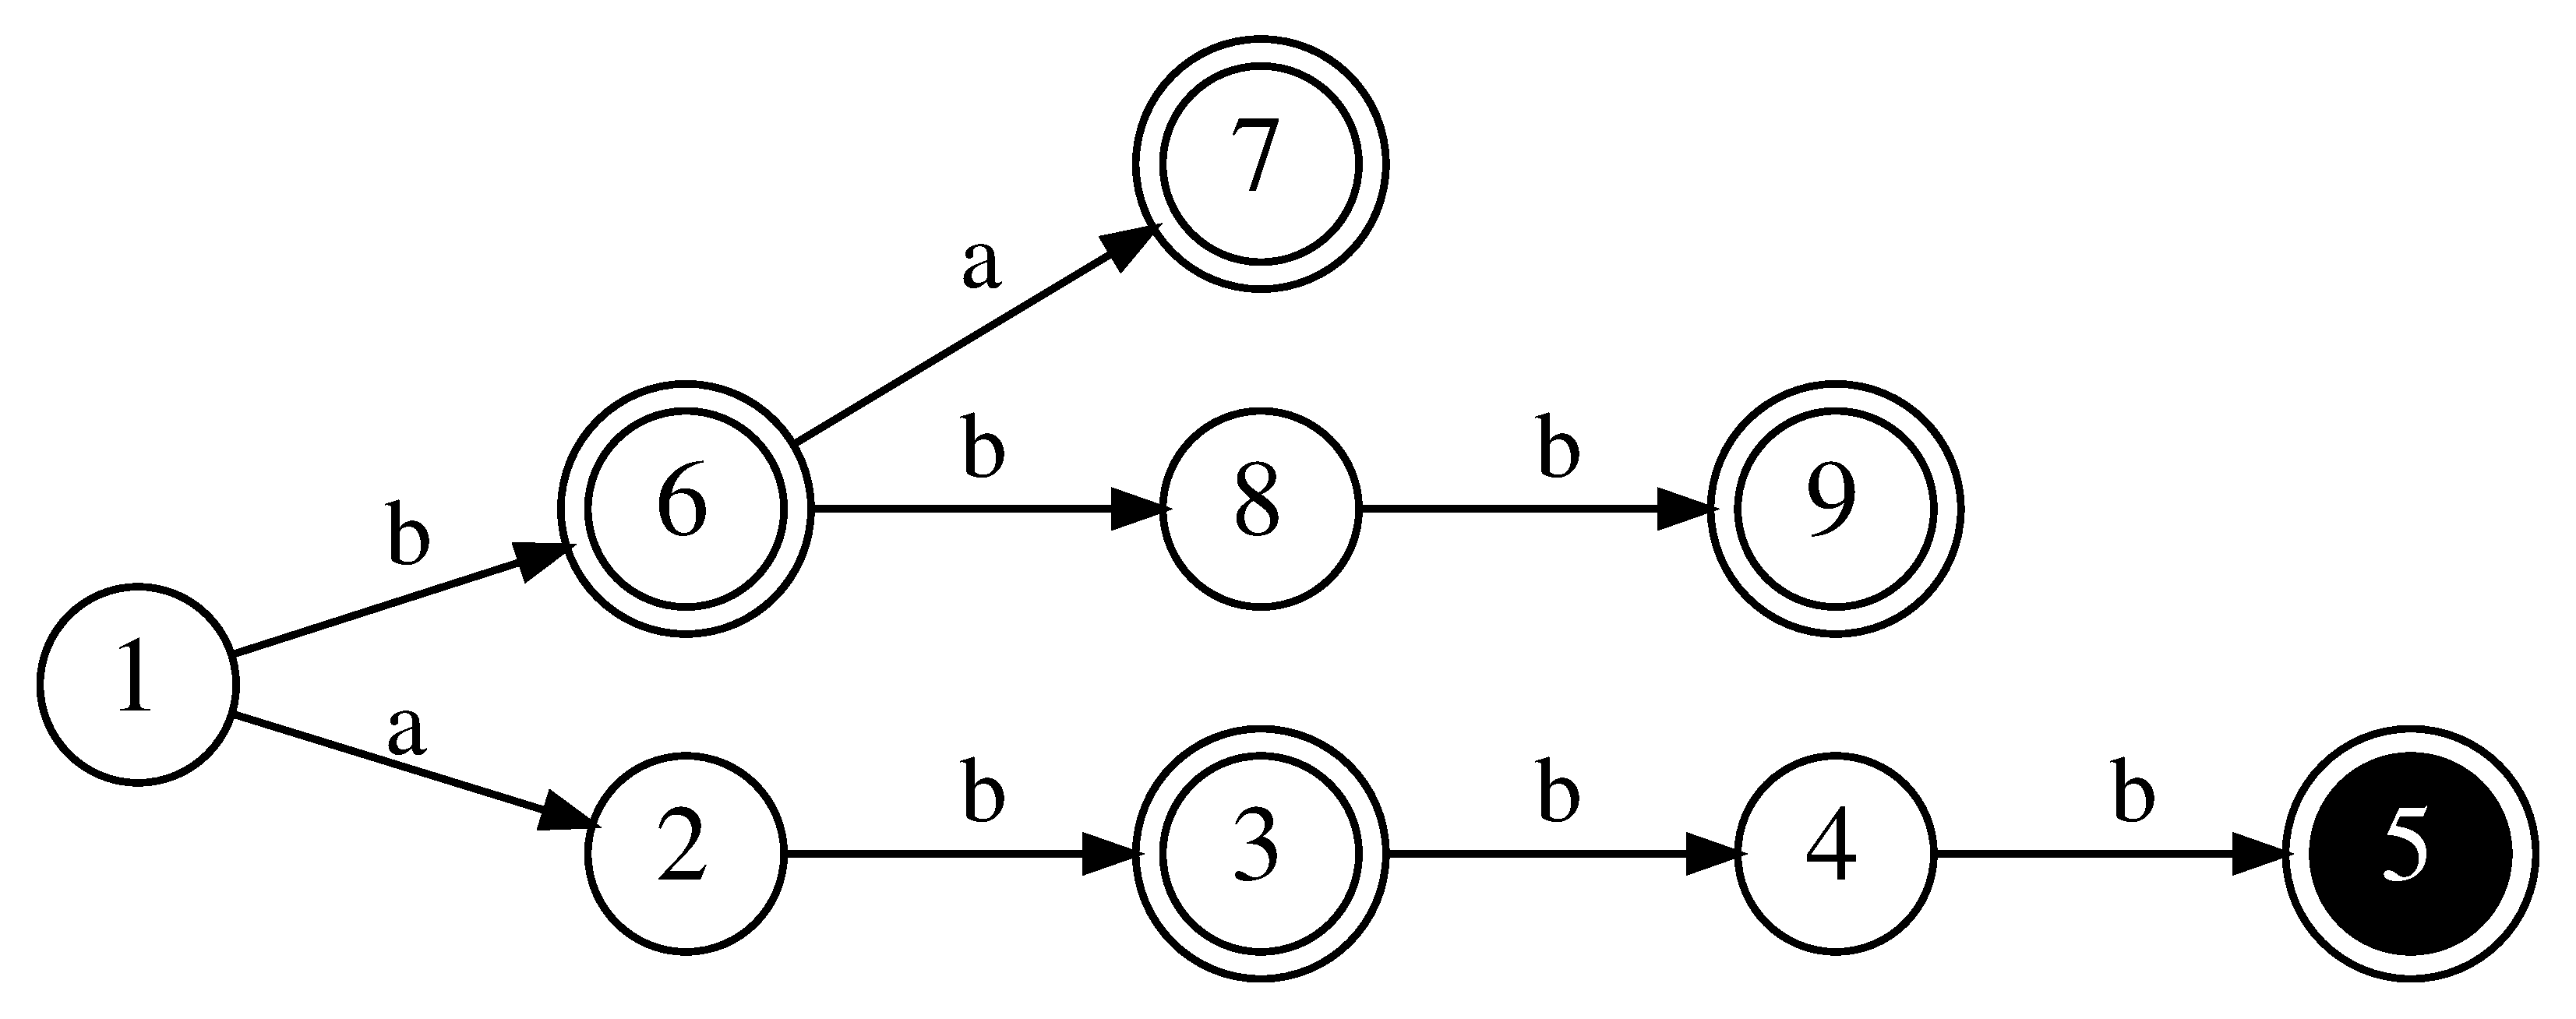
\includegraphics[scale=0.15]{img/datamod/FIG9a.eps}
    \begin{tikzpicture}[
    ->, % makes the edges directed
    >=stealth', % makes the arrow heads bold
    node distance=2cm, % specifies the minimum distance between two nodes. Change if necessary.
    every state/.style={thick, fill=gray!10, minimum size = 0pt}, % sets the properties for each ’state’ node
    initial text=$ $, % sets the text that appears on the start arrow
    double distance between line centers=2pt
]
    \def\yshift{0.47cm}
    \def\xshift{0.26cm}

    \node[state, initial] (q1) {$1$};
    \node[state, accepting] (q6) [above right of=q1, yshift=-\yshift, xshift=\xshift] {$6$};
    \node[state] (q8) [right of=q6] {$8$};
    \node[state, accepting] (q9) [right of=q8] {$9$};
    \node[state] (q2) [below right of=q1, yshift=\yshift, xshift=\xshift] {$2$};
    \node[state, accepting] (q3) [right of=q2] {$3$};
    \node[state] (q4) [right of=q3] {$4$};
    \node[state, fill=white, dashed, inner sep=9.7pt] (q5) [right of=q4] {};
    \node[state, inner sep=4.2pt] (dummy5) [right of=q4] {$5$};
    \node[state, accepting] (q7) [above of=q8, yshift=-0.78cm] {$7$};

    \path
        (q1) edge [above] node {b} (q6)
        (q6) edge [below] node {b} (q8)
        (q8) edge [below] node {b} (q9)
        (q6) edge [above] node {a} (q7)
        (q1) edge [below] node {a} (q2)
        (q2) edge [below] node {b} (q3)
        (q3) edge [below] node {b} (q4)
        (q4) edge [below] node {b} (q5)
        ;
\end{tikzpicture}
  \else
    \begin{tikzpicture}[
    ->, % makes the edges directed
    >=stealth', % makes the arrow heads bold
    node distance=1.5cm, % specifies the minimum distance between two nodes. Change if necessary.
    every state/.style={thick, fill=gray!10, minimum size = 0pt}, % sets the properties for each ’state’ node
    initial text=$ $, % sets the text that appears on the start arrow
]
    \def\yshift{0.36cm}
    \def\xshift{0.2cm}

    \node[state, initial] (q1) {$1$};
    \node[state, accepting] (q6) [above right of=q1, yshift=-\yshift, xshift=\xshift] {$6$};
    \node[state] (q8) [right of=q6] {$8$};
    \node[state, accepting] (q9) [right of=q8] {$9$};
    \node[state] (q2) [below right of=q1, yshift=\yshift, xshift=\xshift] {$2$};
    \node[state, accepting] (q3) [right of=q2] {$3$};
    \node[state] (q4) [right of=q3] {$4$};
    \node[state, dashed, inner sep=7pt] (q5) [right of=q4] {};
    \node[state, inner sep=3pt] (dummy5) [right of=q4] {$5$};
    \node[state, accepting] (q7) [above of=q8, yshift=-0.58cm] {$7$};

    \path
        (q1) edge [above] node {b} (q6)
        (q6) edge [below] node {b} (q8)
        (q8) edge [below] node {b} (q9)
        (q6) edge [above] node {a} (q7)
        (q1) edge [below] node {a} (q2)
        (q2) edge [below] node {b} (q3)
        (q3) edge [below] node {b} (q4)
        (q4) edge [below] node {b} (q5)
        ;
\end{tikzpicture}
  \fi
  \caption{Пример расширенного префиксного дерева для множеств слов $S_{+}=\left\{ab,b,ba,bbb\right\}$ и $S_{-}=\left\{abbb\right\}$}
  \label{img:apta-loop}
\end{figure}
%
На рисунке~\ref{img:dfa-loop} представлен ДКА минимального размера, соответствующий расширенному префиксному дереву, изображенному на рисунку~\ref{img:apta-loop}.
Переход из состояния $2$ по символу $a$ в данном автомате не покрывается никакими переходами префиксного дерева, а значит является свободным.
С помощью предложенных ранее ограничений можно зафиксировать данный переход в виде петли, что продемонстрировано на рисунке штриховой линией.
%
\begin{figure}[ht]
  \centering
  \ifafour
  % 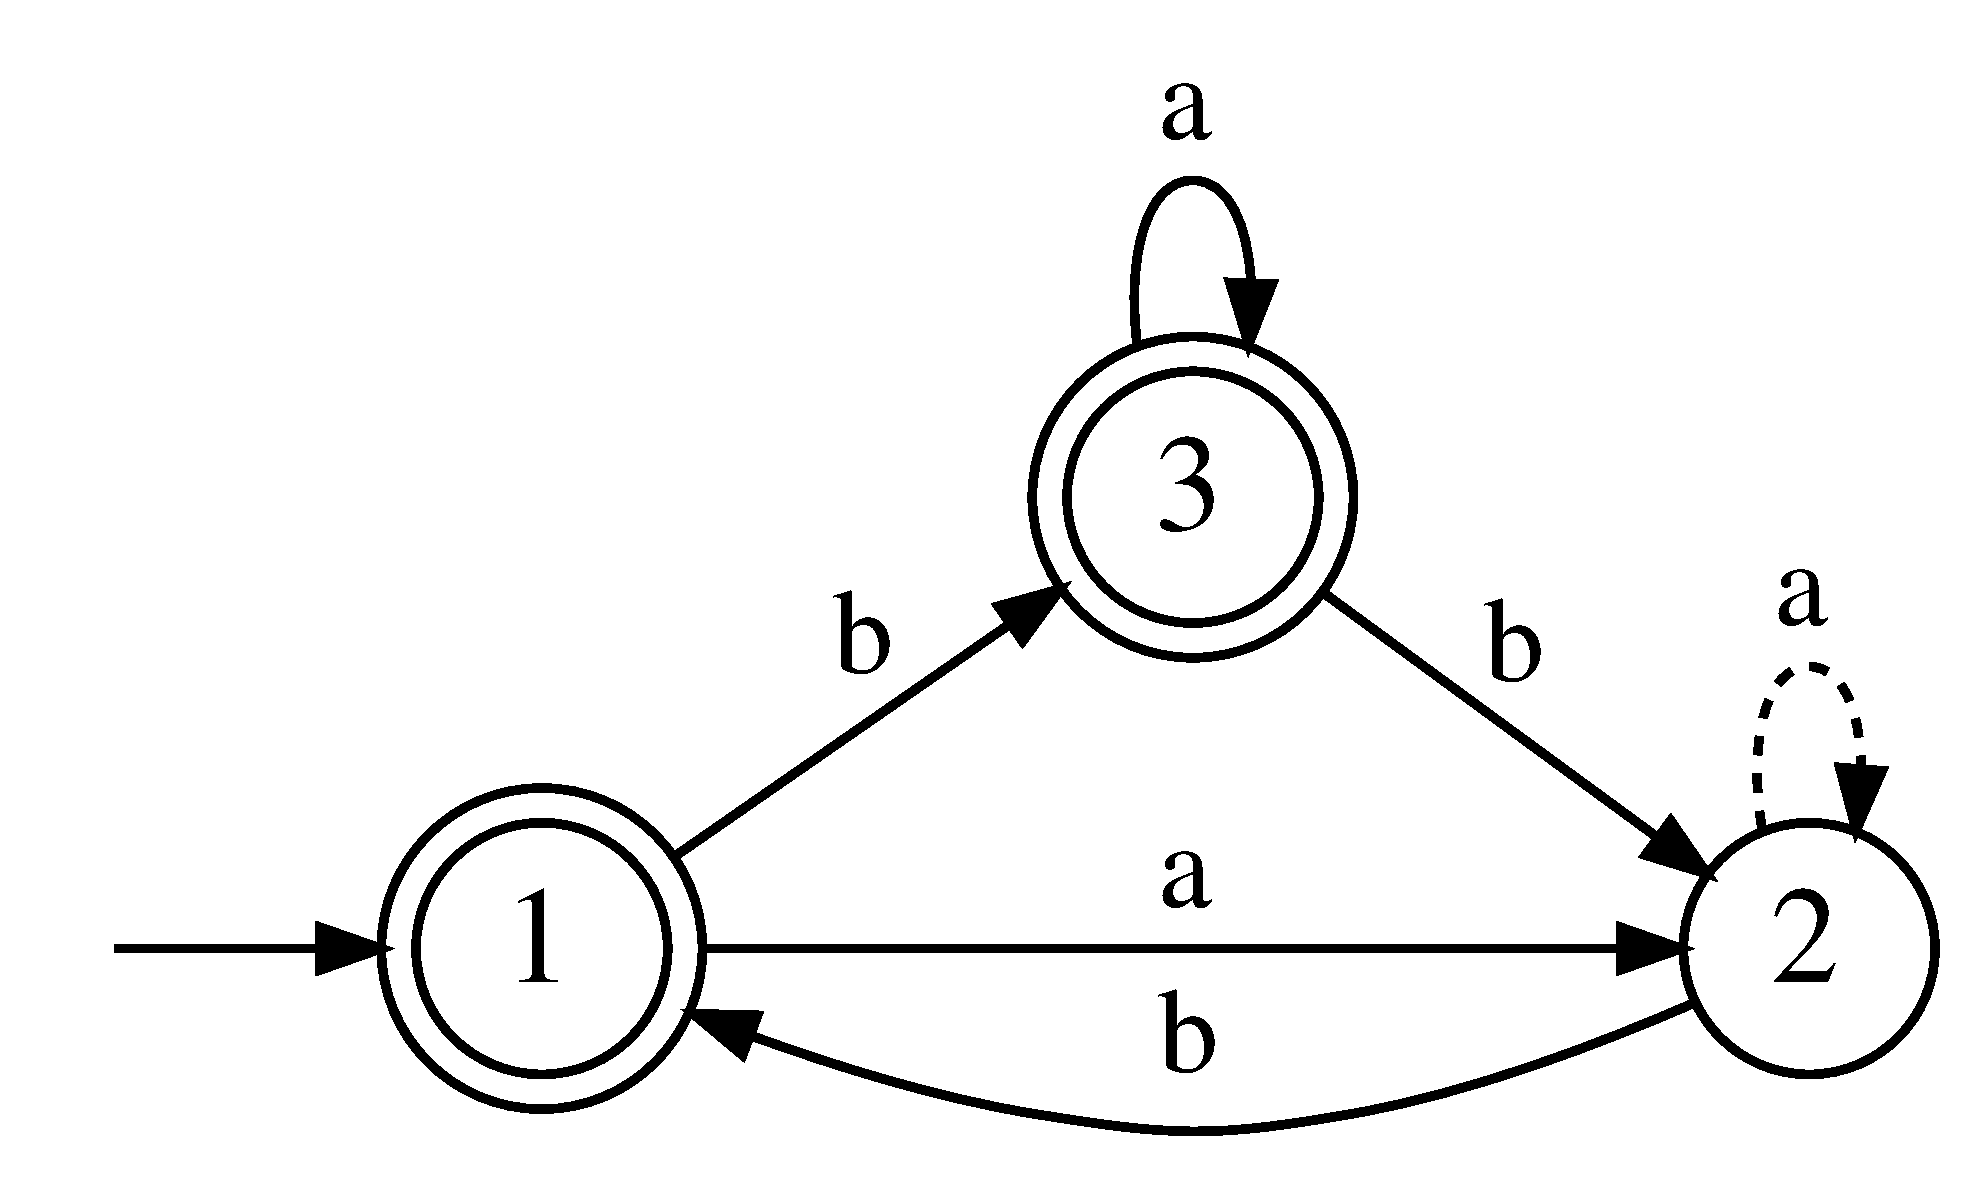
\includegraphics[scale=0.15]{img/datamod/FIG9b.eps}
    \begin{tikzpicture}[
    ->, % makes the edges directed
    >=stealth', % makes the arrow heads bold
    node distance=2.5cm, % specifies the minimum distance between two nodes. Change if necessary.
    every state/.style={thick, fill=gray!10, minimum size = 0pt}, % sets the properties for each ’state’ node
    initial text=$ $, % sets the text that appears on the start arrow
    double distance between line centers=2pt
]
    \node[state, initial, accepting] (q1) {$1$};
    \node[state, accepting] (q3) [above of=q1, xshift=2.5cm/2, yshift=-0.4cm] {$3$};
    \node[state] (q2) [right of=q1] {$2$};

    \path
        (q1) edge [bend right=10, below] node {a} (q2)
        (q2) edge [bend right=10, above] node {b} (q1)
        (q1) edge [left] node {b} (q3)
        (q3) edge [above] node [xshift=2pt] {b} (q2)
        (q2) edge [loop above, dashed] node {a} (q2)
        (q3) edge [loop above] node {a} (q3)
        ;
\end{tikzpicture}
  \else
    \begin{tikzpicture}[
    ->, % makes the edges directed
    >=stealth', % makes the arrow heads bold
    node distance=1.9cm, % specifies the minimum distance between two nodes. Change if necessary.
    every state/.style={thick, fill=gray!10, minimum size = 0pt}, % sets the properties for each ’state’ node
    initial text=$ $, % sets the text that appears on the start arrow
]
    \node[state, initial, accepting] (q1) {$1$};
    \node[state, accepting] (q3) [above of=q1, xshift=1.9cm/2, yshift=-0.3cm] {$3$};
    \node[state] (q2) [right of=q1] {$2$};

    \path
        (q1) edge [bend right=10, below] node {a} (q2)
        (q2) edge [bend right=10, above] node {b} (q1)
        (q1) edge [left] node {b} (q3)
        (q3) edge [above] node [xshift=2pt] {b} (q2)
        (q2) edge [loop above, dashed] node {a} (q2)
        (q3) edge [loop above] node {a} (q3)
        ;
\end{tikzpicture}
  \fi
  \caption{Пример ДКА, построенного по префиксному дереву, представленному на рисунке~\ref{img:apta-loop}, с зафиксированным свободным переходом из состояния $2$ по символу $a$}
  \label{img:dfa-loop}
\end{figure}

%----------------------------------------------------------------------------------------

\section{Реализация и экспериментальные исследования разработанных методов}
\label{sec:findall:results}

В настоящем разделе приводятся описание реализации разработанных методов и экспериментальные исследования, проведенные с ними.

%----------------------------------------------------------------------------------------

\paragraph*{Алгоритм перебора с возвратами.}
\label{sec:findall:results:backtracking}

Так как ранее не предлагалось методов для поиска всех возможных примеров поведения по заданным словарям, то был разработан переборный алгоритм с возвратами, не использующий никаких сторонних программных средств.
Данный алгоритм работает следующим образом.
Изначально создается псевдоДКА $\mathcal{D}$ с $M$ вершинами (где $M$~--- размер искомого ДКА), но без переходов и без выделенных допускающих состояний, который затем будет достраиваться до полноценного ДКА.
Для этого на каждой итерации алгоритма поддерживается фронт расширенного префиксного дерева $\mathcal{A}$ $frontier$~--- множество ребер префиксного дерева $A$, для которых все предшествующие ребра на пути от корня дерева до них уже представлены в автомате $\mathcal{D}$, а они сами~--- еще нет.
Изначально фронт состоит из всех исходящих из корня дерева $\mathcal{A}$ ребер.
Рекурсивная функция $\mathtt{backtracking}$ поддерживает фронт в актуальном состоянии.
Если фронт не пуст, тогда данная функция пытается достроить текущий ДКА с помощью одного из ребер фронта.
После каждого достраивания текущий автомат проверяется на соответствие префиксному дереву, и, если противоречий не найдено, то фронт обновляется.
Если же фронт пуст, то все ребра префиксного дерева $\mathcal{A}$ представленны в автомате $\mathcal{D}$, а значит соответствующий автомат найден.
Тогда ДКА $\mathcal{D}$ проверяется на полноту, и, если автомат не полон, то недостающие переходы добавляются в виде петель (аналогично тому, как это предлагалось делать в предыдущем разделе с помощью переменных использования) с помощью функции $\mathtt{makeComplete}$.
Псевдокод разработанного метода представлен в листинге~\ref{algo:backtracking}.
Функция $\mathtt{findNewFrontier}$ возвращает новый фронт для дополненного ДКА или $\mathtt{NULL}$, если ДКА не соответствует расширенному префиксному дереву.
Данный алгоритм полного поиска основан на алгоритме из~\cite{DBLP:journals/sttt/UlyantsevBS18}.


\begin{algorithm}[ht]
  \caption{Переборный алгоритм с возвратами для генерации всех ДКА минимального размера}
  \label{algo:backtracking}
  \begin{algorithmic}[0]
    \Require расширенное префиксное дерево $\mathcal{A}$; %
    текущая версия искомого ДКА $\mathcal{D}$; %
    фронт $frontier$.
    \Ensure множество $S$ всех неизоморфных ДКА, соответствующих префиксному дереву $\mathcal{A}$.
    \\\hrulefill
    \Function{backtracking}{$\mathcal{A}, \mathcal{D}, frontier$}
      \State $S \gets \text{пустое множество}$
      \State $edge edge \gets \text{любое ребро из } frontier$
      \ForAll{$destination \in 1 \ldots \mathcal{D}.size$}
        \State $source \gets \text{состояние }\mathcal{D}\text{, которому соответствует } edge.from$
        \State $\mathcal{D'} \gets \mathcal{D} \cup \Call{transition}{source, destination, edge.label}$
        \State $frontier' \gets \Call{findNewFrontier}{\mathcal{A}, \mathcal{D'}, frontier}$
        \If{$frontier' \ne \mathtt{NULL}$}
          \If{$frontier' = \emptyset$}
            \State $S.add\left(\Call{makeComplete}{\mathcal{D'}}\right)$
          \Else
            \State $S.add\left(\Call{backtracking}{\mathcal{A}, \mathcal{D'}, frontier'}\right)$
          \EndIf
        \EndIf
      \EndFor
      \Return{$S$}
    \EndFunction
  \end{algorithmic}
\end{algorithm}

%----------------------------------------------------------------------------------------

\paragraph*{Реализация разработанных методов генерации всех детерминированных конечных автоматов.}
\label{sec:findall:results:impl}

Предложенный в предыдущем разделе метод генерации ДКА минимального размера на основе сведения к SAT и с использованием подхода уточнения абстракции по контрпримерам был реализован на языке \emph{python} как модуль программного комплекса \texttt{DFA-Inductor-py}.
Для использования данного метода необходимо указать параметр ``\texttt{--find-all/-all}''.
Также, с помощью параметра ``\texttt{--find-k/-find}'' можно указать число ДКА, которые необходимо сгенерировать.
Любые реализованные предикаты нарушения симметрии и граф несовместимости могут использоваться совместно с данным методом.
Метод генерации ДКА по избыточному набору примеров поведения, использующий подход уточнения абстракции, также может использоваться совместно с данным методом для генерации всех неизоморфных ДКА по избыточному набору примеров поведения.

%----------------------------------------------------------------------------------------

\paragraph*{Экспериментальные исследования разработанных методов генерации всех детерминированных конечных автоматов.}
\label{sec:findall:results:dfs}

Все эксперименты проводились на сервере с 64-ядерным процессором \texttt{AMD Opteron 6378 @ 2.4 ГГц} и операционной системой \texttt{Ubuntu 14.04}.
Для генерации тестовых данных снова использовался алгоритм, предложенный в разделе~\ref{sec:space:results:random-input}.
Использовались следующие параметры: размер искомого автомата $M \in \left[5; 15\right]$, мощность алфавита $L = 2$, суммарное число примеров поведения $S \in \left\{5 \times M; 10 \times M; 25 \times M\right\}$.
Для каждого набора параметров генерировалось по 100 различных автоматов и соответствующих наборов примеров поведения.

Сравнивались три метода генерации всех неизоморфных ДКА по примерам поведения:
\begin{itemize}
  \item метод, основанный на сведении к SAT, из раздела~\ref{sec:findall:SAT-based} с перезапуском программного средства для решения SAT (столбец REST в таблице);
  \item метод, основанный на сведении к SAT, из раздела~\ref{sec:findall:SAT-based} с использованием инкрементального программного средства для решения SAT (INC);
  \item переборный метод с возвратами из раздела~\ref{sec:findall:results:backtracking} (BTR).
\end{itemize}
Результаты экспериментальных исследований представлены в таблице~\ref{tab:find-all}.
Ограничение по времени было установлено в один час (3600 секунд).
Столбец $>$1 показывает процент экземпляров задачи, где существовало больше одного неизоморфного автомата.
Так как в таблице представленно медианное время, то если менее 50 (то есть менее половины) экземпляров были решены, то в соответствующей ячейке стоит прочерк (---).

\begin{table}[ht]
  \centering
  \caption{Медианное время нахождения всех различных ДКА с помощью метода на основе сведения к SAT с перезапуском программного средства (REST), метода на основе сведения к SAT с использованием инкрементального программного средства (INC) и переборного метода с возвратами (BTR)}
  \scalebox{0.65}{
    \begin{tabular}{ccccccccccccccc}
      \hline
      \multirow{2}{*}{$M$} & \multicolumn{4}{c}{$S = 5 \times M$}  & ~ & \multicolumn{4}{c}{$S = 10 \times M$} & ~ & \multicolumn{4}{c}{$S = 25 \times M$}\\\cline{2-5}\cline{7-10}\cline{12-15}
         & $>$1& REST &  INC    & BTR            & & $>$1& REST  & INC  & BTR             & & $>$1& REST & INC  & BTR            \\\hline
      5  & 53  & 2,3   & 2,0   & 0,8            & & 40  & 3,6   & 3,3  & 1,3             & & 17  & 4,1  & 3,4  & 1,5           \\ 
      6  & 56  & 2,8   & 2,4   & 2,1            & & 31  & 4,7   & 3,9  & 1,7             & & 27  & 5,4  & 4,3  & 1,7           \\ 
      7  & 87  & 3,9   & 2,5   & 4,1            & & 27  & 3,7   & 3,0  & 3,1             & & 13  & 7,4  & 6,7  & 2,5          \\ 
      8  & 80  & 4,6   & 3,7   & 87,2           & & 34  & 7,0   & 6,5  & 41,7            & & 16  & 10,1  & 8,9 & 11,6 \\ 
      9  & 91  & 7,6   & 3,9   & 475,1          & & 50  & 7,7   & 6,4  & 121,6           & & 10  & 13,8 & 13,0 & 61,4 \\ 
      10 & 89  & 15,7  & 5,3   & 2756,2         & & 47  & 8,6   & 7,0  & 974,7           & & 11  & 18,8 & 16,1 & 276,8 \\
      11 & 94  & 19,9  & 7,3   & ---             & & 63  & 18,5  & 13,8 & 3108,0          & & 9   & 24,5 & 21,9 & 1158,4 \\
      12 & 90  & 28,0  & 9,9   & ---             & & 49  & 22,3  & 16,7 & ---              & & 8   & 33,5 & 27,2 & 3289,1 \\
      13 & 92  & 185,5 & 18,1  & ---             & & 57  & 36,9  & 22,6 & ---              & & 12  & 62,0 & 51,4 & --- \\
      14 & 87  & 408,5 & 49,0  & ---             & & 71  & 85,1  & 41,8 & ---              & & 4   & 67,0 & 56,2 & --- \\
      15 & 95  & 571,1 & 174,1 & ---             & & 69  & 193,3 & 95,7 & ---              & & 6   & 29,2 & 26,2 & --- \\
      \hline
    \end{tabular}
  }
  \label{tab:find-all}
\end{table}

Результаты экспериментов позволяют сделать несколько выводов.
Во-первых, впервые успешно решена задача генерации всех различных ДКА минимального размера по заданным примерам поведения.
Во-вторых, оба метода, использующие сведение к SAT, значительно превосходят по производительности переборный метод.
В-третьих, использование инкрементального программного средства, как и предполагалось, дает заметное преимущество относительно подхода с перезапуском программного средства, что объясняется сохранением промежуточного состояния инкрементальным программным средством после нахождения некоторого ДКА.
В-четвертых, чем больше примеров поведения дано для генерации ДКА, тем реже случается ситуация, когда существует несколько различных ДКА, соответствующих им.
Однако, надо заметить, что помимо количества примеров поведения, их качество не менее важно.


%----------------------------------------------------------------------------------------

\chresults{\ref{sec:findall}}

В четвертой главе была дана постановка задачи генерации всех неизоморфных ДКА, удовлетворяющих заданным примерам поведения, а также предложен метод решения поставленной задачи.
Разработанный метод был реализован в рамках программного средства \texttt{DFA-Inductor-py}.

Детерминированный конечный автомат минимального размера является максимально точным обобщением имеющихся данных, выраженных с помощью примеров поведения.
Однако в случае, когда примеры поведения недостаточно хорошо описывают искомый автомат, может существовать несколько различных неизоморфных удовлетворяющих автоматов минимального размера.
В таком случае рациональным решением может быть построение всех таких автоматов.
Также, с помощью метода генерации всех ДКА, можно доказать единственность автомата с минимальным числом состояний, соответствующего заданным примерам поведения.
Единственность ДКА в таком случае говорит о том, что имеющиеся данные хорошо описывают найденный автомат.

Без использования предикатов нарушения симметрии на основе кодирования алгоритма BFS или DFS не представляется возможным написать эффективный метод генерации всех неизоморфных ДКА, так как для любого ДКА существует $\mathcal{O}\left(M!\right)$ изоморфных автоматов.
Использование BFS-предикатов нарушения симметрии позволяет оставить единственного представителя для каждого класса эквивалентности по изоморфизму.
Был реализован метод, использующие такие предикаты, для генерации всех неизоморфных ДКА минимального размера.
Экспериментальные исследования показали, разработанный метод демонстрирует значительно меньшее время генерации ДКА относительно реализованного алгоритма перебора с возвратами.
Также, использование программных средств для решения SAT в итеративном режиме позволяет значительно повысить эффективность разработанного метода, так как между вся накопленная информация сохраняется между запусками программного средства.
Все результаты данной главы опубликованы в статье~\cite{zakirzyanov2017DataMode}.


